\documentclass[12pt,a4paper,twoside,openright]{report}
\let\openright=\cleardoublepage



%%% Choose a language %%%

\newif\ifEN
\ENtrue   % uncomment this for english
%\ENfalse   % uncomment this for czech

%%% Configuration of the title page %%%

\def\ThesisTitleStyle{mff} % MFF style
%\def\ThesisTitleStyle{cuni} % uncomment for old-style with cuni.cz logo
%\def\ThesisTitleStyle{natur} % uncomment for nature faculty logo

\def\UKFaculty{Faculty of Mathematics and Physics}
%\def\UKFaculty{Faculty of Science}

\def\UKName{Charles University in Prague} % this is not used in the "mff" style

% Thesis type names, as used in several places in the title
%\def\ThesisTypeTitle{\ifEN BACHELOR THESIS \else BAKALÁŘSKÁ PRÁCE \fi}
\def\ThesisTypeTitle{\ifEN MASTER THESIS \else DIPLOMOVÁ PRÁCE \fi}
%\def\ThesisTypeTitle{\ifEN RIGOROUS THESIS \else RIGORÓZNÍ PRÁCE \fi}
%\def\ThesisTypeTitle{\ifEN DOCTORAL THESIS \else DISERTAČNÍ PRÁCE \fi}
%\def\ThesisGenitive{\ifEN bachelor \else bakalářské \fi}
\def\ThesisGenitive{\ifEN master \else diplomové \fi}
%\def\ThesisGenitive{\ifEN rigorous \else rigorózní \fi}
%\def\ThesisGenitive{\ifEN doctoral \else disertační \fi}
%\def\ThesisAccusative{\ifEN bachelor \else bakalářskou \fi}
\def\ThesisAccusative{\ifEN master \else diplomovou \fi}
%\def\ThesisAccusative{\ifEN rigorous \else rigorózní \fi}
%\def\ThesisAccusative{\ifEN doctoral \else disertační \fi}



%%% Fill in your details %%%

% (Note: \xxx is a "ToDo label" which makes the unfilled visible. Remove it.)
\def\ThesisTitle{Asynchronous Duet Benchmarking}
\def\ThesisAuthor{Tomáš Drozdík}
\def\YearSubmitted{2022}

% department assigned to the thesis
\def\Department{Department of Distributed and Dependable Systems}
% Is it a department (katedra), or an institute (ústav)?
\def\DeptType{Department}

\def\Supervisor{Vojtěch Horký}
\def\SupervisorsDepartment{Department of Distributed and Dependable Systems}

% Study programme and specialization
\def\StudyProgramme{Software Systems}
\def\StudyBranch{\xxx{study branch}}

\def\Dedication{%
Dedication. \xxx{It is nice to say thanks to supervisors, friends, family, book authors and food providers.}
}

\def\AbstractEN{%
\xxx{Abstracts are an abstract form of art. Use the most precise, shortest sentences that state what problem the thesis addresses, how it is approached, pinpoint the exact result achieved, and describe the applications and significance of the results. Highlight anything novel that was discovered or improved by the thesis. Maximum length is 200 words, but try to fit into 120. Abstracts are often used for deciding if a reviewer will be suitable for the thesis; a well-written abstract thus increases the probability of getting a reviewer who will like the thesis.}
% ABSTRACT IS NOT A COPY OF YOUR THESIS ASSIGNMENT!
}

\def\AbstractCS{%
\xxx{You will need to submit both Czech and English abstract to the SIS, no matter what language you use in the thesis. If writing in English, translate the contents of \texttt{\textbackslash{}AbstractEN} into this field. In case you do not speak czech, your supervisor should be able to help you with the translation.}
}

% 3 to 5 keywords (recommended), each enclosed in curly braces.
% Keywords are useful for indexing and searching for the theses by topic.
\def\Keywords{%
\xxx{{key} {words}}
}

% If your abstracts are long and do not fit in the infopage, you can make the
% fonts a bit smaller by this setting. (Also, you should try to compress your abstract more.)
% Alternatively, consider increasing the size of the page by uncommenting the
% geometry modification in thesis.tex.
\def\InfoPageFont{}
%\def\InfoPageFont{\small}  %uncomment to decrease font size

\ifEN\relax\else
% If you are writing a czech thesis, you additionally need to fill in the
% english translation of the metadata here!
\def\ThesisTitleEN{\xxx{Thesis title in English}}
\def\DepartmentEN{\xxx{Name of the department in English}}
\def\DeptTypeEN{\xxx{Department}}
\def\SupervisorsDepartmentEN{\xxx{Superdepartment}}
\def\StudyProgrammeEN{\xxx{study programme}}
\def\StudyBranchEN{\xxx{study branch}}
\def\KeywordsEN{%
\xxx{{key} {words}}
}
\fi


\usepackage[a-2u]{pdfx}

\ifEN\else\usepackage[czech,shorthands=off]{babel}\fi
\usepackage[utf8]{inputenc}
\usepackage[T1]{fontenc}

% See https://en.wikipedia.org/wiki/Canons_of_page_construction before
% modifying the size of printable area. LaTeX defaults are great.
% If you feel it would help anything, you can enlarge the printable area a bit:
%\usepackage[textwidth=390pt,textheight=630pt]{geometry}
% The official recommendation expands the area quite a bit (looks pretty harsh):
%\usepackage[textwidth=145mm,textheight=247mm]{geometry}

%%% FONTS %%%
\usepackage{lmodern} % TeX "original" (this sets up the latin mono)

% Optionally choose an override for the main font for typesetting
\usepackage[mono=false]{libertinus} % popular for comp-sci (ACM uses this)
%\usepackage{tgschola} % Schoolbook-like (gives a bit of historic feel)
%\usepackage[scale=0.96]{tgpagella} % Palladio-like (popular in formal logic).

% Optionally choose a custom sans-serif fonts (e.g. for figures and tables).
% Default sans-serif font is usually Latin Modern Sans. Some font packages
% (e.g. libertinus) replace that with a better matching sans-serif font.
%\usepackage{tgheros} % recommended and very readable (Helvetica-like)
%\usepackage{FiraSans} % looks great
% DO NOT typeset the main text in sans-serif font!
% The serifs make the text easily readable on the paper.

% IMPORTANT FONT NOTE: Some fonts require additional PDF/A conversion using
% the pdfa.sh script. These currently include only 'tgpagella'; but various
% other fonts from the texlive distribution need that too (mainly the Droid
% font family).


% some useful packages
\usepackage{amsmath,amsfonts,amsthm,bm}
\usepackage{graphicx}
\usepackage{xcolor}
\usepackage{booktabs}
\usepackage{caption}
\usepackage{floatrow}

% load bibliography tools
\usepackage[backend=bibtex,natbib,style=numeric,sorting=none]{biblatex}
% alternative with alphanumeric citations (more informative than numbers):
%\usepackage[backend=bibtex,natbib,style=alphabetic]{biblatex}
%
% alternatives that conform to iso690
% (iso690 is not formally required on MFF, but may help elsewhere):
%\usepackage[backend=bibtex,natbib,style=iso-numeric,sorting=none]{biblatex}
%\usepackage[backend=bibtex,natbib,style=iso-alphabetic]{biblatex}
%
% additional option choices:
%  - add `giveninits=true` to typeset "E. A. Poe" instead of full Edgar Allan
%  - `terseinits=true` additionaly shortens it to nature-like "Poe EA"
%  - add `maxnames=10` to limit (or loosen) the maximum number of authors in
%    bibliography entry before shortening to `et al.` (useful when referring to
%    book collections that may have hundreds of authors)
%  - for additional flexibility (e.g. multiple reference sections, etc.),
%    remove `backend=bibtex` and compile with `biber` instead of `bibtex` (see
%    Makefile)
%  - `sorting=none` causes the bibliography list to be ordered by the order of
%    citation as they appear in the text, which is usually the desired behavior
%    with numeric citations. Additionally you can use a style like
%    `numeric-comp` that compresses the long lists of citations such as
%    [1,2,3,4,5,6,7,8] to simpler [1--8]. This is especially useful if you plan
%    to add tremendous amounts of citations, as usual in life sciences and
%    bioinformatics.
%  - if you don't like the "In:" appearing in the bibliography, use the
%    extended style (`ext-numeric` or `ext-alphabetic`), and add option
%    `articlein=false`.
%
% possibly reverse the names of the authors with the default styles:
%\DeclareNameAlias{default}{family-given}

% load the file with bibliography entries
\addbibresource{refs}

% remove this if you won't use fancy verbatim environments
\usepackage{fancyvrb}

% remove this if you won't typeset TikZ graphics
\usepackage{tikz}
\usetikzlibrary{positioning} %add libraries as needed (shapes, decorations, ...)

% remove this if you won't typeset any pseudocode
\usepackage{algpseudocode}
\usepackage{algorithm}

% remove this if you won't list any source code
\usepackage{listings}


\hypersetup{unicode}
\hypersetup{breaklinks=true}

\usepackage[noabbrev]{cleveref}


% various forms of TODOs (you should remove this before submitting)
\usepackage[textsize=tiny, backgroundcolor=yellow!25, linecolor=black!25]{todonotes}
\newcommand{\xxx}[1]{\textcolor{red!}{#1}}

 % remove this before compiling the final version


% use this for typesetting a chapter without a number, e.g. intro and outro
\def\chapwithtoc#1{
\chapter*{#1}
\addcontentsline{toc}{chapter}{#1}
}

% If there is a line/figure overflowing into page margin, this will make the
% problem evident by drawing a thick black line at the overflowing spot. You
% should not disable this.
\overfullrule=3mm

% The maximum stretching of a space. Increasing this makes the text a bit more
% sloppy, but may prevent the overflows by moving words to next line.
\emergencystretch=2em

\ifEN
\theoremstyle{plain}
\newtheorem{thm}{Theorem}
\newtheorem{lemma}[thm]{Lemma}
\newtheorem{claim}[thm]{Claim}
\newtheorem{defn}{Definition}
\theoremstyle{remark}
\newtheorem*{cor}{Corollary}
\else
\theoremstyle{plain}
\newtheorem{thm}{Věta}
\newtheorem{lemma}{Lemma}
\newtheorem{claim}{Tvrzení}
\newtheorem{defn}{Definice}
\theoremstyle{remark}
\newtheorem*{cor}{Důsledek}
\fi

\newenvironment{myproof}{
  \par\medskip\noindent
  \textit{\ifEN Proof \else Důkaz \fi}.
}{
\newline
\rightline{$\qedsymbol$}
}

% real/natural numbers
\newcommand{\R}{\mathbb{R}}
\newcommand{\N}{\mathbb{N}}

% asymptotic complexity
\newcommand{\asy}[1]{\mathcal{O}(#1)}

% listings and default lstlisting config (remove if unused)
\DeclareNewFloatType{listing}{}
\floatsetup[listing]{style=ruled}

\DeclareCaptionStyle{thesis}{style=base,font={small,sf},labelfont=bf,labelsep=quad}
\captionsetup{style=thesis}
\captionsetup[algorithm]{style=thesis,singlelinecheck=off}
\captionsetup[listing]{style=thesis,singlelinecheck=off}

% Uncomment for table captions on top. This is sometimes recommended by the
% style guide, and even required for some publication types.
%\floatsetup[table]{capposition=top}
%
% (Opinionated rant:) Captions on top are not "compatible" with the general
% guideline that the tables should be formatted to be quickly visually
% comprehensible and *beautiful* in general (like figures), and that the table
% "head" row (with column names) should alone communicate most of the content
% and interpretation of the table. If you just need to show a long boring list
% of numbers (because you have to), either put some effort into showing the
% data in an attractive figure-table, or move the data to an attachment and
% refer to it, so that the boredom does not impact the main text flow.
%
% You can make the top-captions look much less ugly by aligning the widths of
% the caption and the table, with setting `framefit=yes`, as shown below.  This
% additionally requires some extra markup in your {table} environments; see the
% comments in the example table in `ch2.tex` for details.
%\floatsetup[table]{capposition=top,framefit=yes}

\ifEN\floatname{listing}{Listing}
\else\floatname{listing}{Výpis kódu}\fi
\lstset{ % use this to define styling for any other language
  language=C++,
  tabsize=2,
  showstringspaces=false,
  basicstyle=\footnotesize\tt\color{black!75},
  identifierstyle=\bfseries\color{black},
  commentstyle=\color{green!50!black},
  stringstyle=\color{red!50!black},
  keywordstyle=\color{blue!75!black}}

% Czech versions of the used cleveref references (It's not as convenient as in
% English because of declension, cleveref is limited to sg/pl nominative. Use
% plain \ref to dodge that.)
\ifEN\relax\else
\crefname{chapter}{kapitola}{kapitoly}
\Crefname{chapter}{Kapitola}{Kapitoly}
\crefname{section}{sekce}{sekce}
\Crefname{section}{Sekce}{Sekce}
\crefname{subsection}{sekce}{sekce}
\Crefname{subsection}{Sekce}{Sekce}
\crefname{subsubsection}{sekce}{sekce}
\Crefname{subsubsection}{Sekce}{Sekce}
\crefname{figure}{obrázek}{obrázky}
\Crefname{figure}{Obrázek}{Obrázky}
\crefname{table}{tabulka}{tabulky}
\Crefname{table}{Tabulka}{Tabulky}
\crefname{listing}{výpis}{výpisy}
\Crefname{listing}{Výpis}{Výpisy}
\floatname{algorithm}{Algoritmus}
\crefname{algorithm}{algoritmus}{algoritmy}
\Crefname{algorithm}{Algoritmus}{Algoritmy}
\newcommand{\crefpairconjunction}{ a~}
\newcommand{\crefrangeconjunction}{ a~}
\fi

\newcommand\vh[1]{\marginpar[$\clubsuit$]{$\clubsuit$}{\color{red}\textbf{VH:} #1 $\square$}}
 % use this file for various custom definitions


\begin{document}

% the layout is mandatory, edit only in dire circumstances

\pagestyle{empty}
\hypersetup{pageanchor=false}
\begin{center}

% top part of the layout, this actually differs between faculties

\def\ThesisTitleXmff{%
  \ifEN
    \centerline{\mbox{
\includegraphics[width=166mm]{img/logo-en.pdf}}}
  \else
    \centerline{\mbox{
\includegraphics[width=166mm]{img/logo-cs.pdf}}}
  \fi
  \vspace{-8mm}\vfill%
  {\bf\Large\ThesisTypeTitle}
  \vfill%
  {\LARGE\ThesisAuthor}\par
  \vspace{15mm}%
  {\LARGE\bfseries\ThesisTitle}
  \vfill%
  \Department}
\def\ThesisTitleCuniLogo#1{%
  {\large\UKName\par\medskip\par\UKFaculty }
  \vfill%
  {\bf\Large\ThesisTypeTitle}
  \vfill%
  \includegraphics[width=70mm]{#1}
  \vfill%
  {\LARGE\ThesisAuthor}\par
  \vspace{15mm}%
  {\LARGE\bfseries\ThesisTitle}
  \vfill%
  \Department\par}
\def\ThesisTitleXcuni{\ThesisTitleCuniLogo{img/uklogo.pdf}}
\def\ThesisTitleXnatur{\ThesisTitleCuniLogo{img/naturlogo.pdf}}

% choose the correct page and print it
\csname ThesisTitleX\ThesisTitleStyle\endcsname
% latex corner: X is the new @

\vfill

{
\centerline{\vbox{\halign{\hbox to 0.45\hsize{\hfil #}&\hskip 0.5em\parbox[t]{0.45\hsize}{\raggedright #}\cr
\ifEN Supervisor of the \ThesisGenitive thesis:
\else Vedoucí \ThesisGenitive práce: \fi
& \Supervisor \cr
\noalign{\vspace{2mm}}
\ifEN Study programme: \else Studijní program: \fi
& \StudyProgramme \cr
\noalign{\vspace{2mm}}
\ifEN Study branch: \else Studijní obor: \fi
& \StudyBranch \cr
}}}}

\vfill

\ifEN Prague \else Praha \fi
\YearSubmitted

\end{center}

\newpage

% remember to sign this!
\openright
\hypersetup{pageanchor=true}
\pagestyle{plain}
\pagenumbering{roman}
\vglue 0pt plus 1fill

\ifEN
\noindent
I declare that I carried out this \ThesisAccusative thesis independently, and only with the cited
sources, literature and other professional sources. It has not been used to obtain another
or the same degree.
\else
\noindent
Prohlašuji, že jsem tuto \ThesisAccusative práci vypracoval(a) samostatně a výhradně
s~použitím citovaných pramenů, literatury a dalších odborných zdrojů.
Tato práce nebyla využita k získání jiného nebo stejného titulu.
\fi

\ifEN
\medskip\noindent
I understand that my work relates to the rights and obligations under the Act No.~121/2000 Sb.,
the Copyright Act, as amended, in particular the fact that the Charles
University has the right to conclude a license agreement on the use of this
work as a school work pursuant to Section 60 subsection 1 of the Copyright~Act.
\else
\medskip\noindent
Beru na~vědomí, že se na moji práci vztahují práva a povinnosti vyplývající
ze zákona č. 121/2000 Sb., autorského zákona v~platném znění, zejména skutečnost,
že Univerzita Karlova má právo na~uzavření licenční smlouvy o~užití této
práce jako školního díla podle §60 odst. 1 autorského zákona.
\fi

\vspace{10mm}


\ifEN
\hbox{\hbox to 0.5\hsize{%
In \hbox to 6em{\dotfill} date \hbox to 6em{\dotfill}
\hss}\hbox to 0.5\hsize{\dotfill\quad}}
\smallskip
\hbox{\hbox to 0.5\hsize{}\hbox to 0.5\hsize{\hfil Author's signature\hfil}}
\else
\hbox{\hbox to 0.5\hsize{%
V \hbox to 6em{\dotfill} dne \hbox to 6em{\dotfill}
\hss}\hbox to 0.5\hsize{\dotfill\quad}}
\smallskip
\hbox{\hbox to 0.5\hsize{}\hbox to 0.5\hsize{\hfil Podpis autora\hfil}}
\fi

\vspace{20mm}
\newpage

% dedication

\openright

\noindent
\Dedication

\newpage

% mandatory information page

\openright

\vbox to 0.49\vsize{\InfoPageFont
\setlength\parindent{0mm}
\setlength\parskip{5mm}

\ifEN Title: \else Název práce: \fi
\ThesisTitle

\ifEN Author: \else Autor: \fi
\ThesisAuthor

\DeptType:
\Department

\ifEN Supervisor: \else Vedoucí bakalářské práce: \fi
\Supervisor, \SupervisorsDepartment

\ifEN Abstract: \AbstractEN \else Abstrakt: \AbstractCS \fi

\ifEN Keywords: \else Klíčová slova: \fi
\Keywords

\vss}\ifEN\relax\else\nobreak\vbox to 0.49\vsize{\InfoPageFont
\setlength\parindent{0mm}
\setlength\parskip{5mm}

Title:
\ThesisTitleEN

Author:
\ThesisAuthor

\DeptTypeEN:
\DepartmentEN

Supervisor:
\Supervisor, \SupervisorsDepartmentEN

Abstract:
\AbstractEN

Keywords:
\KeywordsEN

\vss}
\fi

\newpage

\openright
\pagestyle{plain}
\pagenumbering{arabic}
\setcounter{page}{1}


\tableofcontents

\chapwithtoc{Introduction}

% What is the nature of the problem the thesis is addressing?
Modern software development with rapid development cycles is in dire need of a fast, accessible, scalable, and reliable performance regression detection method.
A typical question is if neighboring commits of the same software manifest regression.
For instance, authors of a compiler might be concerned if a new optimization increased the performance of a particular benchmark.

% What is the common approach for solving that problem now?
The traditional method of performance measurement relies on a dedicated bare-metal server with an isolated and carefully set up environment that tries to prevent measurement noise.
This method is reasonably fast and reliable but lacks accessibility and scalability requirements as the cost of maintenance is high.

To address the scalability and accessibility much research over the past decade has focused on offloading performance measurements to the cloud~\cite{leitner2016patterns, laaber2019software, abedi2017conducting}.
Cloud offers scalable \mbox{on-demand} infrastructure with pay for what you use principle.
However, this research has shown that performance measurement in the cloud is difficult because of the high variability of the shared infrastructure environment.

Even in ideally crafted \mbox{bare-metal} conditions, multiple measurements are necessary to deal with the inherent variability introduced by the code running platform, such as \mbox{just-in-time} compilation, garbage collection, memory mapping, and CPU frequency scaling.
Benchmark code itself can have its share of non-determinism that contributes to the overall variability of the measurements.
Hence, in addition to benchmark harness running its workload in a loop practitioners often run the benchmark multiple times.
Afterward, analyze individual iteration scores to evaluate the final score.

In the context of compiler programmers, they may run multiple benchmarks on a version with and without the optimization and compare the final scores.
We refer to this method as \emph{sequential benchmarking} as it runs different versions after each other.

\citet{bulej2020duet} introduced a new benchmarking method called \emph{duet benchmarking} designed with volatile environments such as the cloud in mind.
The main idea of duet benchmarking is to run both versions in parallel.
The distinguishing property of this method is that it does not try to prevent interference, on the contrary, duet benchmarking acknowledges the presence of variability and relies on fair scheduling to make the impact equal on both versions running in parallel.
Afterward, the benchmark scores are statistically evaluated to determine if there is a performance regression between the two versions.
The duet benchmarking method has shown improvement ranging from $5.03 \times$ on average for Scalabench and DaCapo workloads to $37.4 \times$ on average for SPEC CPU 2017 workloads~\cite{bulej2020duet}.
However, this method relies on synchronized iterations of a benchmark, which requires benchmark harness modification that synchronizes individual iterations between harnesses.

% How this thesis approaches the problem?
This thesis explores the relaxation of this synchronization requirement which creates a new variant of the duet method we call \emph{asynchronous duet method}.
To achieve this, we implement a tool for running benchmarks that supports sequential, synchronous, and asynchronous duet methods.
One novel attribute of this tool is that it runs benchmarks in containers to achieve portability and ease of setup.

Using the tool we run benchmarks from multiple benchmarking suites --- Renaissance, Scalabench, DaCapo, and SPEC CPU 2017.
The first three are \mbox{JVM-based} while the last one represents natively compiled benchmarks.
The goal of this thesis is to assess the viability of the asynchronous duet method for different benchmarks across different environments.
Our choice of environments included bare-metal measurements on a dedicated server, AWS EC2 \lstinline{t3.medium} instance as cloud representative, and self-hosted shared virtual machine infrastructure.

% What are the results? Did something improve?
Results show that asynchronous duet performs very similarly to synchronous duet in terms of A/A detection accuracy.
It is also able to achieve minimal detectable slowdowns (MDS)~\cite{laaber2019software} of $1\%$ for SPEC CPU benchmarks and $3-5\%$ for \mbox{JVM-based} benchmarks.
Somewhat unexpectedly, our cloud measurements did not manifest variance much bigger than the \mbox{bare-metal} environment while the shared virtual machine environment came out as the most volatile.

Another surprising result was the performance of the sequential method, which performed well when it comes to the overall variability of iteration scores with a coefficient of variability being lower for many benchmarks.
However, the sequential method did not perform well in the statistical tests we chose for regression detection.

That relates to arguably the biggest advantage of the duet methods which is its overall runtime reduction compared to sequential methods.
Some benchmarks were able to finish in half the time using duet methods compared to sequential methods which directly translates to $50\%$ cost reduction.
Although, the speedup was dependent on the environment.
The cloud environment even experienced some slowdowns, likely due to fewer available CPUs.

% What can the reader expect in the individual chapters of the thesis?
The thesis is structured as follows.
The first chapter provides some background on benchmarking in volatile environments.
The second chapter delves into duet benchmarking and poses research questions for this thesis with the goals summarized at the end of this chapter.
The third chapter describes the architecture of our benchmark automation tool capable of running benchmarks from multiple suites using both sequential and duet methods.
The fourth chapter summarizes the statistical methods used to evaluate regressions which are later used in the fifth chapter that presents the results.
Finally, we conclude the thesis and lay out the possibilities for future work in this area.

\chapter{Background and Motivation}
\label{chap:background}

% Introduce benchmarks
Benchmark harness sets up an environment, executes benchmark code in multiple iterations, and then presents some score.
The score can be iteration time, throughput, number of processed requests etcetera.
When a benchmark is a small piece of code, also referred to as performance unit tests by~\citet{horky2015unit}, it is usually written in some microbenchmark framework.
Microbenchmark execution in a public cloud has been thoroughly examined by~\citet{laaber2019software}.
If the benchmark code gets bigger it is usually referred to as the application benchmark.

% Introduce benchmark suites
Benchmarks do not have the sole purpose of measuring the performance of an application, inversely they provide a way to measure the capabilities of some hardware.
For this reason, benchmark suites aggregate many application workloads, put them under a single harness, and simplify the performance evaluation process.
Examples of such suites are from Standard Performance Evaluation Corporation (SPEC) SPEC CPU \footnote{SPEC CPU® 2017 \url{https://www.spec.org/cpu2017/}} and SPECjbb \footnote{SPECjbb® 2015 \url{https://www.spec.org/jbb2015/}}.
Other standalone suites used in this thesis are Renaissance~\cite{prokopec2019renaissance}, DaCapo \footnote{DaCapo Benchmarks \url{https://dacapo-bench.org/}}, and ScalaBench \footnote{Scala Benchmarking Project \url{https://www.scalabench.org/}} suite.
All above-mentioned suites are Java-based except for SPEC CPU which has benchmarks written in C, C++, and Fortran and hence is natively compiled.
Apart from testing hardware performance, benchmark suites are good candidates for research in performance measurement methods as they strive to provide a wide range of real-world representative workloads.

% Reason about long execution time and attractiveness of the cloud approach
The requirement for multiple repetitions causes an inherent trade-off between accuracy and execution time.
Execution of a benchmark suite for some software project version, with the goal to identify newly introduced performance regression, can take an overwhelming 3000 machine hours per day as analyzed by~\citet{bulej2020duet} on an open-source GraalVM project~\footnote{Oracle. GraalVM repository at GitHub \url{https://github.com/oracle/graal}}.
By then a new version could have come around.
This trade-off between measurement execution time and the number of commits between tested versions can be addressed from multiple angles.
One is to reduce the number of measurements by identification of commits that might introduce performance regression~\citet{oliveira2017perphecy}.
Other is to reduce the execution time of measurements by parallelization.
Effective parallelization involves maintaining multiple dedicated machines which is difficult and costly.
Therefore, much research over the past decade has focused on offloading performance measurements to the cloud~\cite{leitner2016patterns, laaber2019software, abedi2017conducting}.

% Describe the nature of benchmarking in the cloud
\section{Benchmarking in the cloud}
Cloud offers practically infinite hardware scaling capabilities with on-demand access and a \mbox{pay-for-what-you-use} principle.
That makes it a tempting platform for fast and accessible performance measurements.
Cloud offers large scale of options to run your code on from bare metal offerings \footnote{AWS Outposts \url{https://aws.amazon.com/outposts/}} to running small pieces of code as lambdas~\footnote{AWS Lambda \url{https://aws.amazon.com/lambda/}}.
The most commonly examined and accessible method is an \mbox{Infrastructure-as-a-Service} (IaaS) cloud offering where computing resources are acquired and released as a service.

IaaS is typically in form of virtual machines or containers with attached virtual disks.
These are referred to as instances, and they come with different configuration options such as a number of virtual CPUs, size of memory, network throughput, and virtual disk.
This gives practitioners some control over what hardware and software platform is used to run their code compared to higher-level offerings such as Platform-as-a-Service (PaaS) and Software-as-a-Service (SaaS).

% Performance stability in the cloud -~\citet{laaber2019software}.
Studies such as~\citet{leitner2016patterns} and~\citet{laaber2019software} summarize the viability of measuring software performance on IaaS offerings from different providers.
They point out that measuring software performance on the public cloud is very much a moving target with providers constantly changing their offerings, hardware, and processes.
A common concern is that a given instance type may not run on the same type of hardware and that the same physical hardware might host multiple colocated instances.
Hardware heterogeneity, shared and virtualized infrastructure further amplifies the variability of performance measurements in the cloud environment~\cite{leitner2016patterns} even to the point that using state-of-the-art statistical methods and performance measurements practitioners might not be able to detect $1000\%$ slowdown of some measured software as shown by~\citet{laaber2019software}.

% Introduce statistical methods, later on, mention repeatability, cite do we teach useful statistics?
With many repetitions and variability across the results, it is necessary to carefully process the results and use statistical methods to find out if a code change introduces a new performance regression.
The use of statistical methods has been extensively studied in~\citet{bulej2017stat} and further analyzed in~\citet{laaber2019software} specifically in the cloud context.
To quantify the variability of the distribution of results from a benchmark~\citet{laaber2019software} use the coefficient of variance, also called mean standard deviation.
To compare results of two software versions~\citet{bulej2017stat} use both methods of overlapping confidence intervals computed by bootstrap procedure and hypothesis testing with Wilcoxon rank-sum test and its variation Mann-Whiteney U-test as well as Welch's t-test.
\citet{bulej2017stat} also raise concerns about the validity of these methods when used for performance measurement data.
Concerns stem from the fact that performance measurements don't satisfy many common assumptions that statistical methods make such as random independent and identically distributed samples and asymptotic normality of the data.
Moreover, performance data also tend to exhibit long-range dependencies between samples, have unknown distributions with long tails, and are not stationary in general which further complicates statistical analysis~\cite{bulej2017stat}.
So far there does not seem to be any "silver bullet" statistical method that would be a good fit for performance data and thus these techniques need to be used with caution as reasoned in multiple studies~\cite{leitner2016patterns, laaber2019software, bulej2017stat}.

% Measurement methods designed for variable cloud environment
Unfavorable conditions for benchmarking in the cloud spiked interest in research that focuses on performance measurement methods that reduce measurement variability, increase accuracy and reduce false positives of regression detection in a cloud environment.
One such method and current best practice~\cite{laaber2019software} is called \emph{Randomized Multiple Interleaved Trials} (RMIT) introduced by~\citet{abedi2017conducting}.
Trial refers to a single run of benchmark, with multiple inside iterations, on a particular version of the software it measures the performance of.
To compare performance between multiple versions of some software --- alternatives one has to run the same benchmark with each alternative.
RMIT states that these runs of these alternatives should be run (1) multiple times as discussed above and (2) repetitions of all alternatives should be randomized to minimize both partial and periodic outside interference.

Another method that aims to reduce variance is already mentioned duet benchmarking first introduced in~\citet{bulej2019initial} and further expanded on in~\citet{bulej2020duet}.
The next chapter examines the duet method and its new asynchronous variant in detail and poses research goals for this thesis.

\chapter{Duet benchmarking}
\label{chap:duet}

Benchmark comparison between two versions of software is referred to as A/B benchmarking, where A and B are some software versions that run the same benchmark code in multiple iterations.
\Cref{fig:method_timeline} shows comparison between three benchmarking methods analyzed in this thesis (1) sequential, (2) synchronous duet and (3) asynchronous duet.
Sequential method is the simples where each version is run independently of each other.
Synchronous duet on the other hand runs A and B in parallel and it has to synchronize starts of individual iterations.
Asynchronous duet runs in parallel as well but does not require synchronized iterations.

\begin{figure}
	\centering
	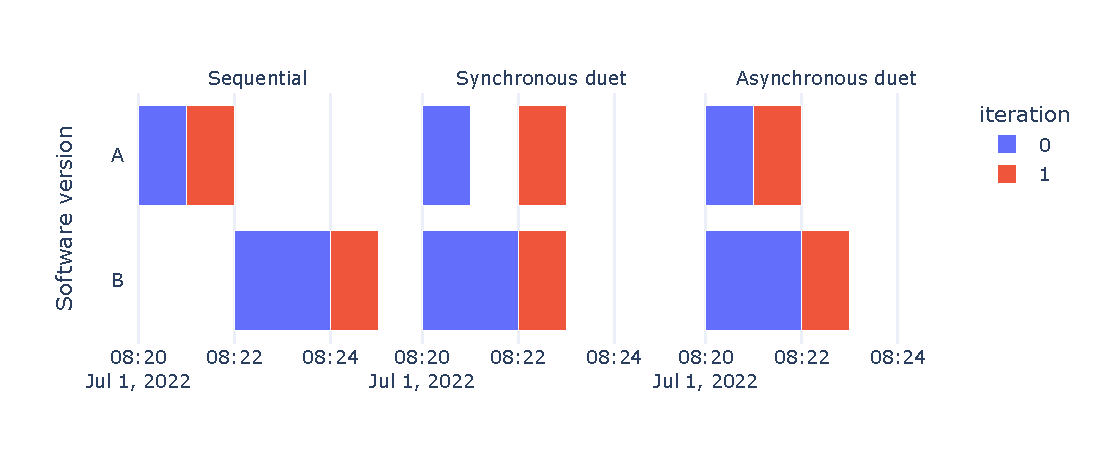
\includegraphics[width=.9\linewidth]{./figures/method_timeline.pdf}
	\caption{
	Comparison of different benchmarking methods sequential, synchronous duet, and asynchronous duet when comparing 2 software versions A and B.
	Benchmark runs 2 iterations with the same durations for all methods and versions.
	Note that version B introduced a regression where first iteration takes twice as long.
	X axes is an example timeline of measurements.
	}
	\label{fig:method_timeline}
\end{figure}

% RQ1 Runtime reduction
This example has the durations of iterations equal for all methods, that illustrates one immediate benefit of running duet benchmarks --- overall runtime reduction.
Ideally duet method could save up to $50\%$ or execution run time and hence halve execution costs.
However, in order to achieve such speedup, workloads running in parallel must not interfere with each other.

\begin{quote}
	\textbf{RQ1:} \emph{What are the runtime savings of duet methods compared to the sequential method?}
\end{quote}

% Mutual interference
To address mutual workload interference,~\citet{bulej2020duet} set up measurements in such a way that each benchmark was restricted to single dedicated virtual core.
Even then, it may be the case that the two virtual cores map to the same hardware threads of the same physical core.
Such virtual cores would then compete for the single shared physical core.
Here~\citet{bulej2019initial} rely on workload symetry which states that if a cloud were to exhibit systematic performance difference between the two virtual cores running duet workloads, it would likely exhibit similar unwarranted performance difference in other common concurrent workloads, such behavior would be likely considered a bug and remedied.
In other words they rely on fair CPU scheduling to work out mutual interference.
\citet{bulej2019initial} also note that this works only for similar workloads, which can be expected of neighboring commits or versions of the same software.

% External interference, Synchronized interference, Impact symetry for seqn syncduet and async duet.

\section{Synchronous vs. Asynchronous duet}

% Impact symetry on asynchronous duet
\Cref{fig:method_timeline} also note that synchronized duet methods are not always running in parallel.
Once an iteration finishes it has to wait for its pair iteration to finish, until then, this pair iteration runs alone.
It might seem that asynchronous duet solves this issue because iterations are not blocked on barrier, so the only iteration running alone will be the last iteration of either A or B, whichever finishes last.

However, asynchronous duet might be worse of in terms of equal impact symetry on parallel workloads due to ways benchmark harnesses and benchmarks themselves work.
\Cref{alg:harness} is a generic example of how inner loop of benchmark harness might look like.
Pre and post iteration functions might do some environment checks like running garbage collection or recording results.
Benchmark harness authors did not have any reason to care of reduced noise around the measured code, nor keep the loop tight.
Therefore it is natural that  asynchronous duet might suffer from this.

\begin{algorithm}
\begin{algorithmic}
	\Function{RunHarness}{$b$}
		\State \Call{Setup}{$b$}
		\For{$i \in 1 \dots I$}
		 	\State \Call{PreIteration}{}
			\State $start \gets$ \Call{clock.now}{}
			\State \Call{RunBenchmark}($b$)
			\State $end \gets$ \Call{clock.now}{}
			\State \Call{PostIteration}{$b$, $i$, $start$, $end$}
		\EndFor
		\State \Call{ValidateResults}{$b$}
		\State \Call{Teardown}{$b$}
	\EndFunction
\end{algorithmic}
\caption{
	Generic workings of the benchmark harness which executes a benchmark.
	Note that not all harnesses follow this structure --- some functions might be effectively empty.
	Specifically for synchronous duet~\citet{bulej2020duet} had to modify \emph{PreIteration} to wait on barrier.
}
\label{alg:harness}
\end{algorithm}

\Cref{fig:overlap_timeline} figure shows what implications can absence of synchronization have on workload overlaps.
With enough iterations, harness specifics, and potentially different A/B performance it is inevitable that workloads will diverge.
Even if workloads are partially overlapping, start of a workload might do different things, for example be CPU bound, compared to the end of the workload, that might be I/O bound.
This further hinders the impact symetry for asynchronous duet that synchronous duet method relies on.

% RQ2 Overlaps
\begin{quote}
	\textbf{RQ2:} \emph{How do workloads overlap in asynchronous duet?}
\end{quote}

\begin{figure}
	\centering
	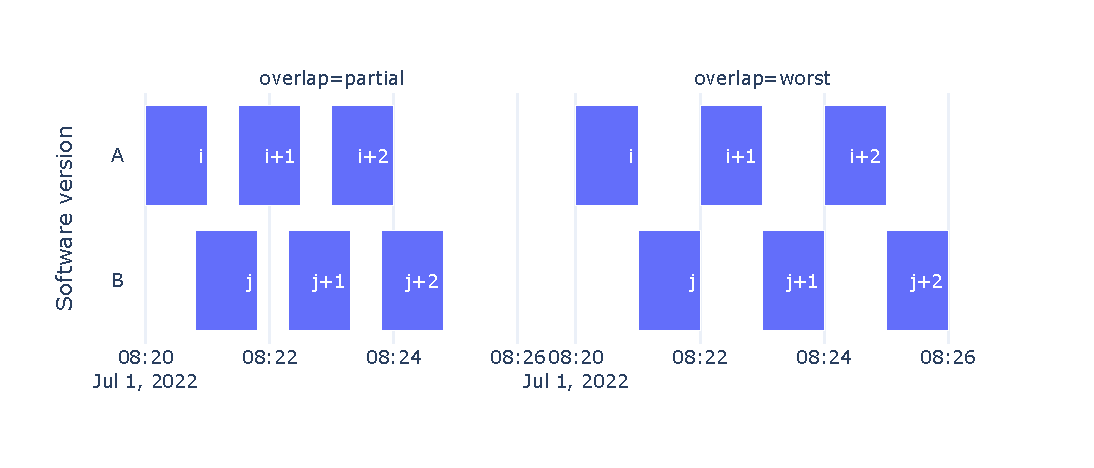
\includegraphics[width=.9\linewidth]{./figures/overlap_timeline.pdf}
	\caption{
		Tailored examples of how lack of synchronization might affect overlap of timed benchmark code.
		This is an example timeline of iterations of an \emph{asynchronous duet} measurement from an iteration $i$ and $j$ for versions $A$ and $B$ respectively.
		Focus on how versions $A$ and $B$ overlap --- just partially or even not at all.
	}
	\label{fig:overlap_timeline}
\end{figure}

For asynchronous duet method to be any useful runtime reduction and overlapping workloads are not enough.
Asynchronous duet method has to show variance improvements on par with the synchronized duet method.

% RQ3 Variable environment
\begin{quote}
	\textbf{RQ3:} \emph{What is the variance of asynchronous-duet compared to synchronous duet and sequential execution across different envrironments?}
\end{quote}

Additionally using similar approach to~\citet{laaber2019software} asynchronous and synchronous duet methods can be compared with sequential measurements in terms of \emph{minimal detectable slowdowns}~\xxx{cref to chap4}.

% RQ4 Minimal detectable slowdown
\begin{quote}
	\textbf{RQ4:} \emph{What are the minimal detectable slowdowns that we can detect with $95\%$ confidence?}
\end{quote}

% Why is it important - runtime reduction, variable environment, no suite modification
To summarize research into duet methods in this thesis focuses on:
\begin{description}
	\item[Runtime and Cost reduction] Duet methods have potential to drastically reduce, up to $50\%$, the execution time of benchmarks.
	\item[Accuracy] Synchronized duet method can reduce variance of benchmark results measured in variable environment, such as public cloud~\citet{bulej2020duet}. Question is if asynchronous duet can do the same?
	\item[Accesibility] Asynchronous duet relaxes synchronized requirement on benchmark harnesses which makes this method more broadly usable.
\end{description}

\chapter{Implementation}
\label{chap:impl}

We implemented a super-harness that takes an existing benchmark harness as an input and executes its benchmarks in the asynchronous duet style.

% Running in docker and reasons for it
To keep a configuration portable and the dependencies minimal we have decided to use the container technology, namely Docker~\cite{merkel2014docker} or Podman~\cite{podman}.
Tool is named \lstinline{duetbench}, and it is part of open sourced python package \lstinline{duet}~\cite{duet} that also implements other complementary tools described in~\cref{sec:result_parsing}.
Documentation is in the form of GitHub wiki~\cite{wiki}.

We want to compare asynchronous duet with~\citet{bulej2020duet}, hence our super-harness supports synchronized duet and sequential method in a containerized environment.

\section{Architecture}

\Cref{fig:duetbench_sequence} depicts architecture of \lstinline{duetbench} script.
\lstinline{duetbench} is a process on the host machine that spawns subprocesses that run containers --- one for each version A/B.
Since initialization of a container might take longer \lstinline{duetbench} waits for both containers to start and then uses \lstinline{docker exec}\footnote{\url{https://docs.docker.com/engine/reference/commandline/exec/}} to run the command that executes the benchmark harness loop from~\cref{alg:harness}.
Once both benchmarks finish, copy the raw result of those benchmarks from their respective containers and store them in a predefined directory structure that preserves super-harness metadata and raw results~\cite{wiki}.
Afterward, stop and clean up both containers.
We refer to this process as a \emph{run} and it is analogous to a \emph{trial} from~\citet{laaber2019software} and~\citet{abedi2017conducting} for sequential runs.
For duet methods, one \emph{run} executes 2 benchmarks in parallel.

\begin{figure}[!ht]
    \centering
    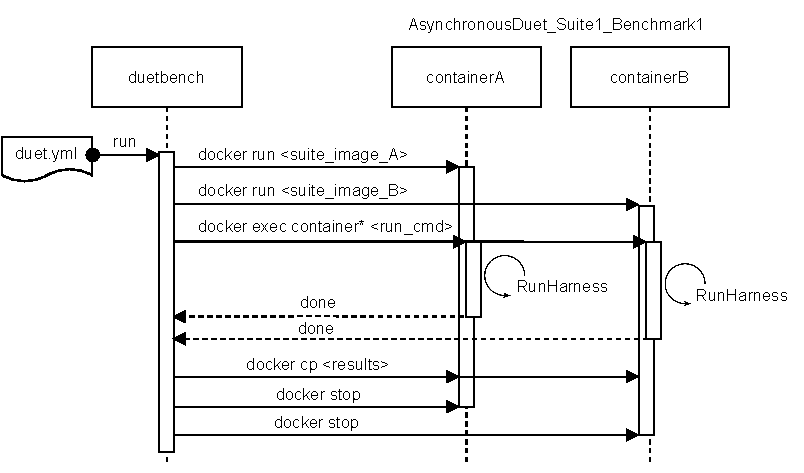
\includegraphics[width=\linewidth]{./figures/duetbench-sequence.drawio.pdf}
    \caption{
        UML sequence diagram of how \lstinline{duetbench} executes a single A/B asynchronous duet benchmark.
        All the parameters in angled brackets are specified in the configuration file \lstinline{duet.yml} described in~\cref{sec:configuration}.
        Note that the docker commands are simplified for brevity.
    }
    \label{fig:duetbench_sequence}
\end{figure}

If there are more benchmarks to execute pick the next one (according to a particular scheduling strategy, see~\cref{sec:scheduling}) and do the same process.
In the case of the sequential method, the process is very much the same just omit the second container entirely and run them separately.

\subsection{Synchronized duet in containerized environment}
\label{sec:sync_duet_impl}

\citet{bulej2020duet} uses a \mbox{shared-memory} barrier to synchronize benchmark iterations.
We ported this solution into the containers to mimic the original behavior.

The barrier uses the pthread API that is not available on all systems such as macOS.
Therefore, \lstinline{duetbench} starts a third container to initialize, and later clean up the barrier, hence bypassing the missing functionality on the host system.

Docker environments are separated by design.
To facilitate this feature \lstinline{duetbench} mounts host directory \lstinline{-v /dev/shm:/dev/shm} and shares \mbox{inter-process} communication namespace \lstinline{--ipc host}\footnote{\url{https://docs.docker.com/engine/reference/run/}}.

\subsection{Run Scheduling}
\label{sec:scheduling}

\lstinline{duetbench} supports two options for \emph{run scheduling}:
\begin{description}
    \item[Sequential] where benchmarks are run in order of definition from a configuration file.
    \item[Randomized Interleaving Trials] where it randomly interleaves the runs from a configuration file.
        Hence, it can mix different types of measurement methods and benchmarks.
        With multiple repetitions of a given measurement method, it is essentially RMIT~\cite{abedi2017conducting}.
\end{description}

\section{Configuration}
\label{sec:configuration}

\Cref{lst:config} shows section of \lstinline{duetbench} YAML configuration file that describes an A/B asynchronous duet and sequential run.
The goal of the design was to make configuration generic and simple to use so that many harnesses and benchmark suites can be adapted to use with \lstinline{duetbench}.
Full documentation of the \lstinline{duetbench} configuration including a description of how to run synchronized duets (not present in the~\cref{lst:config}) is on the wiki~\cite{wiki}.

Freedom in run command allows for tweaking of the harness to better suit asynchronous duet.
For example, some harnesses support skips of validation or various garbage collector options.
Detailed configuration of experiments is in~\cref{sec:experiment_setup}.

\begin{listing}[!ht]
    \begin{lstlisting}
avrora:
  image: dacapo
  duet_repetitions: 2
  sequential_repetitions: 2
  schedule: randomized_interleaving_trials
  A:
    run: java -jar dacapo-A.jar -n 50 -o results.csv avrora
  B:
    run: java -jar dacapo-B.jar -n 50 -o results.csv avrora
  results:
    - results.csv
    \end{lstlisting}
    \caption{
        Example part of YAML configuration file for \lstinline{duetbench} that runs \lstinline{avrora} benchmark from the DaCapo suite.
        In this case, both A and B versions are packaged in a single container image as Java JAR archives.
        Run command specifies how to invoke the DaCapo harness --- 50 iterations, results in \lstinline{results.csv} and run only \lstinline{avrora} benchmark.
        All the result files or directories need to be specified in \lstinline{results} array field.
        Note the correspondence between user input fields from this configuration and parameters in angled brackets from~\cref{fig:duetbench_sequence}.
        Furthermore, users can specify the number of repetitions for both asynchronous duet and sequential measurements, as well as the scheduling strategy for those runs.
    }
    \label{lst:config}
\end{listing}

\section{Result parsing}
\label{sec:result_parsing}

Once a run finishes, results are copied in their raw format to a dedicated result directory on the host machine.
Results are then processed using \lstinline{duetprocess} script~\cite{wiki} for further analysis.
\lstinline{duetprocess} takes an output directory of \lstinline{duetbench} as input and produces a single CSV result file.

The minimal schema of a result data point looks like this:
\begin{itemize}
    \item Directly parsed by \lstinline{duetprocess}:
        \begin{itemize}
            \item suite,
            \item benchmark,
            \item run --- repetition id, not necessary in  order of execution,
            \item pair,
            \item pair order --- which pair was started first,
            \item iteration,
            \item \emph{artifacts} --- \lstinline{duetbench} provides an option to run some additional commands such as \lstinline{lscpu} or \lstinline{cat /proc/meminfo} to obtain information about host environment.
        \end{itemize}
    \item Specific per benchmark suite parsers:
        \begin{itemize}
            \item iteration start absolute timestamp,
            \item iteration end absolute timestamp.
        \end{itemize}
\end{itemize}

Since different benchmark suites have widely different results formats users have to write a parser plugin --- python function.
The parser has to obtain iteration start and end absolute timestamps from benchmark results. 
Additionally, since users need to write a parser for a given benchmark suite, they might add any sort of data that the benchmark produces as an addition to the above-mentioned schema.

Some benchmark suites don't track absolute timestamps of iterations and thus need some modification.
However, without absolute timestamps, one could not evaluate how iterations overlap (\emph{RQ2}).

\subsection{Notation}
\label{sec:notation}

To describe parsed results more formally and describe terminology from the \lstinline{duet} package we use the following terms:

\begin{description}
    \item[Environment] $e \in E$ classifies host hardware and software configuration --- where \lstinline{duetbench} runs.
        The environment is deduced from artifacts in the above schema.
        The set of environments $E$ used in our experiments is described in~\cref{sec:experiment_setup}.
    \item[Type] $t \in T$ is the measurement method type where $T = \{seqn, sduet, aduet\}$ for sequential, synchronous duet and asynchronous duet respectively.
    \item[Pair] $p \in P$ is version of tested software in case of A/B runs $P = \{A, B\}$
    \item[Benchmark] $b \in B$ is a benchmark from a benchmark suite, formally $B = \{(suite, benchmark)~|~benchmark \in suite \}$
    \item[Run] in environment $e \in E$ of type $t \in T$ running benchmark $b \in B$ and pair $p \in P$ is denoted as $R^{e, t, b, p}$.
        It is a unit that \lstinline{duetbench} works with and can run multiple times.
    \item[Iterations] of a run $R^{e, t, b, p}$ with $iters$ iterations is an ordered set $(i_1, i_2, \dots i_{iters})$ of scores of particular benchmark --- execution time in nanoseconds.
\end{description}

To distinguish different measurement methods for some benchmark $b \in B$ in an environment $e \in E$ denote a set of all sequential runs as
\begin{align*}
M^{e, b}_{seqn} &= \{(R^{e, seqn, b, A}_r,~R^{e, seqn, b, B}_r)~|~\forall r \in \{1 \dots runs\}\},
\end{align*}

set of all synchronized duet measurements which are naturally paired on the level of pairs and iterations as
\begin{align*}
M^{e, b}_{sduet} &= \{(R^{e, sduet, b, A}_r,~R^{e, sduet, b, B}_r)~|~\forall r \in \{1 \dots runs\}\}\\
                 &= \{(i^A_j,~i^B_j)_r~|~\forall r \in \{1 \dots runs\},~\forall j \in \{1 \dots iters\}\},
\end{align*}

and finally set of all asynchronous duet measurements, naturally paired on the level of pairs as
\begin{align*}
M^{e, b}_{aduet} &= \{(R^{e, aduet, b, A}_r,~R^{e, aduet, b, B}_r)~|~\forall r \in \{1 \dots runs\}\}.
                 %&= \{((i_j)^A,~(i_j)^B)_r~|~~r \in \{1 \dots runs\},~j \in \{1 \dots iters\}\},
\end{align*}

Finally, refer to $M^e$ as the union of all runs in an environment $e \in E$
$$
M^e = \{ M^{e, b}_{seqn} \cup M^{e, b}_{sduet} \cup M^{e, b}_{aduet} ~|~ b \in B \}.
$$


\subsection{Overlaps}
\label{sec:overlaps}

To address \emph{RQ2} \lstinline{duetprocess} provides a method to compute overlaps of iterations of a given asynchronous duet run.
Let $(R^A, R^B) \in M^{e, b}_{aduet}$.
Iterations of respective runs are $R^A = (i^A_1 \dots i^A_{iters})$ and $R^B = (i^B_1 \dots i^B_{iters})$.
To define iteration overlaps the following notation is used:
\begin{align*}
start(i) &= \text{start of iteration } i,\\
end(i) &= \text{end of iteration } i,\\
overlap\_start(i^A, i^B) &= max(start(i^A), start(i^B)),\\
overlap\_end(i^A, i^B) &= min(end(i^A), end(i^B)).
\end{align*} 
Then set of overlaps of these two runs $O_{R^A, R^B}$ can be expressed as
\begin{align*}
O_{R^A, R^B} =&~\{(i^A_j, i^B_k)~|~overlap\_start(i^A_j, i^B_k) < overlap\_end(i^A_j, i^B_k),\\
              &~~\forall j \in \{1 \dots iters\}, \forall k \in \{1 \dots iters\}\}.
\end{align*} 

However, not all overlaps are equally important.
As shown in~\cref{fig:overlap_timeline} and \emph{RQ2} introduction, some overlaps might be tiny and cover the start of one iteration with the end of another.
The following notations are used to express the quality of an overlap:
\begin{align*}
overlap\_time(i^A, i^B) &= overlap\_end(i^A, i^B) - overlap\_start(i^A, i^B), \\
overlap\_rate^A(i^A, i^B) &= \frac{overlap\_time(i^A, i^B)}{i^A}, \\
overlap\_rate^B(i^A, i^B) &= \frac{overlap\_time(i^A, i^B)}{i^B}, \\
overlap\_rate(i^A, i^B) &= min(overlap\_rate^A(i^A, i^B), overlap\_rate^B(i^A, i^B)).
\end{align*}

Denote a set of all asynchronous duet overlaps for a benchmark $b \in B$ in an environment $e \in E$ as
$$
O^{e,b} = \{O_{R^A, R^B}~|~(R^A, R^B) \in M^{e,b}_{aduet}\}.
$$

\chapter{Overview of Results Processing}
\label{chap:results}

With multiple repetitions and inherent variance of measurements statistical analysis is used to determine performance regression in an A/B run.
This chapter describes statistical methods we use to determine and compare measurement variance and regression detection of an A/B run using different benchmarking methods.

\section{A/A runs}

Finding a software project that exhibits certain slowdown is difficult since regression is often tied to the hardware running the benchmark.
Instead, research into performance measurements employs A/A measurement technique~\cite[laaber2019software, bulej2020duet].
A/A measurement runs the same version and later labels runs with A and B labels --- as if there were 2 different versions.
Since the code is the same the performance should be the same as well.
Usability of a benchmarking method can thus be a result of its ability to correctly detect A/A measurements correctly.
In the context of duet runs A/B labeling is performed on concurrently running duet pairs.

\section{Data filtering}
\label{sec:data_filtering}

In our experiments, we removed the first half of all iterations per run of \mbox{JVM-based} benchmarks to avoid warm-up, same as in~\citet{bulej2020duet}.
% TODO: \citet{horky2015java} note that detecting warm-ups is difficult \xxx{read what is says about warm up}.
\xxx{TODO: describe that we did not remove anything from SpecCPU.}

\section{Accuracy analysis and performance regression tests}

\xxx{TODO: this sentence feels like its repeating what has been said already.}
The goal of benchmarking is to determine performance speedup or a regression.
The high variance of iteration times makes this more difficult, but the synchronous duet method has shown \xxx{variance improvements from XYZ to XYZ}~\citet{bulej2020duet}.
To address the variance of benchmarking methods, using containers, across different environments (\emph{RQ3}), we use various statistical methods.

\subsection{Relative standard deviation}
\label{sec:cv}

Relative standard deviation, also known as the coefficient of variation ($CV$), is one way to determine the variance of iteration times.
For measurement type $t \in T$, benchmark $b \in B$, runs $R^{t, b} \in M^e$:
\begin{align*}
CV^{t, b} &= \frac{std(R^{t, b})}{mean(R^{t, b})} = \frac{std(\{i~|~i \in R^{t, b}\})}{mean(\{i~|~i \in R^{t, b}\})}
\end{align*}

The $CV$ is a measure of how the results of different benchmarks vary relative to each other using different benchmarking methods.
However, the variance of duet methods cannot be determined just based on $CV$.

For instance, higher $CV$ for given benchmark's duet measurements compared to its sequential measurements doesn't imply worse predictability of duet methods because of the impact symmetry argument.
Overall variance might be higher, but the pairwise comparison could be more telling.
On the other hand, lower $CV$ for duet methods suggests better robustness of duet methods.

\subsection{Confidence interval test}
\label{sec:ci_test}

To determine if pairs manifest performance change use the method of confidence intervals from~\citet{bulej2020duet}.
This method also provides a variance comparison across benchmarking methods based on relative confidence interval width.
Here, we describe the method and extend its use for the asynchronous duet.

First, runs and their iterations need to be paired.
\begin{description}
    \item[Sequential] runs don't have any natural pairing but are randomly paired by the nature of A/A runs labeling. We decided to pair their iterations sequentially
        $$
        is\_pair(i^A_i, i^B_j) = i == j
        $$
    \item[Synchronous duet] runs are naturally paired - sequentially by iterations, thus they have the same $is\_pair$ predicate.
    \item[Asynchronous duet] runs can't be paired sequentially.
        Considering A/B measurements, non-synchronized iterations will inevitably diverge, hence sequential iteration pairing wouldn't support impact symmetry.
        Instead, we decided to pair iterations $i^A$ and $i^B$ based on the minimum overlap ratio $m \in (0, 1)$ and thus define a set of filtered overlaps as
        $$
        O^{e,b}_m = \{(i^A, i^B)~|~(i^A, i^B) \in O^{e, b}, overlap\_rate(i^A, i^B) > m\}.
        $$
        The smaller the $m$, the fewer pairs of iterations there will be and vice versa.
        It follows that this is a predicate for asynchronous duet pairing with minimum overlap ratio parameter $m$
        $$
        is\_pair(i^A, i^B) = (i^A, i^B) \in O^{e,b}_m.
        $$
        Analysis of how many overlaps there are for different $m$s is in~\cref{sec:rq2}.
\end{description}
Each pairing method returns a set of paired iterations for an experiment $M^{e, b}_t$,
$$
Pairs(M^{e, b}_t) = \{(i^A, i^B)~|~is\_pair(i^A, i^B),~\forall~i^A, i^B \in M^{e, b}_t\}.
$$

Second, paired iteration times are subtracted to determine the difference between all pairs which yields random sample $X$ with distribution $F_X$
$$
X = \{i^A - i^B~|~(i^A, i^B)~\in~Pairs(M^{e, b}_t)\}.
$$

Furthermore, \citet{bulej2017stat} recommend to use \emph{run means} sampling instead of \emph{runs merged} sampling.
The runs merged method uses all paired iterations from all runs as a sample.
Run means, on the other hand, aggregates paired iterations in a paired run using statistical methods, for example, arithmetic mean and uses those as samples.
Given $r$ runs each with $i$ iterations \emph{runs merged} results in $r * i$ observations and \emph{run means} results in $r$ observations.

These observations are used to create $95\%$ confidence interval using non-parametric bootstrap with $9999$ draws with replacement and arithmetic mean as statistics.~\footnote{We used the bootstrap method from python \lstinline{scipy} package \url{https://docs.scipy.org/doc/scipy/reference/generated/scipy.stats.bootstrap.html} that uses a \mbox{bias-corrected} and accelerated method to compute the CI by default.}
For A/A runs we expect distribution $F_X$ to be centered around~$0$.
Therefore, if the confidence interval encompasses~$0$, we consider the workloads equal, otherwise report a difference.
 
\subsubsection{Variability comparison using CI}
\label{sec:ci_width}

Another use of these confidence intervals is to compute their relative width and compare the variance of different measurement methods~\cite{bulej2019initial}.
$$
CI_{relative\_width}(X) = \frac{CI_{width}(X)}{mean(X)}.
$$

\subsection{Mann-Whitney u-test}
\label{sec:utest}

The next method to evaluate regression in an A/B run is to use hypothesis testing.
One such test used for purpose of A/B performance evaluation is Mann-Whitney \mbox{u-test}~\cite{bulej2017stat,laaber2019software}.
It is a non-parametric test of the null hypothesis that two samples come from the same distribution.
One sample is the iteration durations of pair A and the other is of pair B.

We used \mbox{u-test} implementation from \lstinline{scipy} python package~\footnote{\url{https://docs.scipy.org/doc/scipy/reference/generated/scipy.stats.mannwhitneyu.html}} in its two-sided variant and decide to reject the null hypothesis if \mbox{p-value} is less than $5\%$.
Hence, if \mbox{p-value} is below $5\%$ for a given benchmark, test method, and environment reject the null hypothesis --- sample distributions are distinct enough, thus we report a performance change.

\section{Minimal detectable slowdown}
\label{sec:mds}

%Same as in~\citet{laaber2019software}, caveats with the overlaps.
\Citet{laaber2019software} explore the minimal detectable slowdowns (MDS) for a sequential micro-benchmarking method to determine which micro-benchmarks are viable for cloud benchmarking.
We use this method to determine the viability of duet methods compared to sequential methods in the cloud environment.

First, A/A test results need to be adjusted --- emulate a scenario where pair B is $s$ times wlog slower --- emulating A/B test results where version B has a performance regression.
For all iterations running version B, multiply its runtime by $s$.
$$
\forall (R^A, R^B) \in M^{e} ~:~ R^B_{slowed} = \{i * s~|~\forall i \in R^B \}.
$$\
For asynchronous duet increased iteration times of B affect the overlap of A and B.
Thus we need to recompute the start and end timestamps of each B's iteration, assuming the gaps in between workload runs remain unchanged.

Second, use either the confidence interval test or \mbox{Mann-Whitney} \mbox{u-test} to determine if adjusted A/B measurements show performance regression on different known slowdowns.

\chapwithtoc{Conclusion}

Our main goal was to evaluate the behavior of a new duet method variant that does not synchronize iterations.
Particularly we wanted to answer questions from~\cref{sec:goals}.

% Was the problem stated in the introduction solved? (Ideally include a list of successfully achieved goals.)
%% Accessibility
First of which was better accessibility of duet methods.
We achieved that by creating a benchmark super-harness tool that can run benchmarks from multiple suites in a portable containerized way using both sequential and duet methods.
This tool was used to run measurements in cloud, bare-metal and shared virtual machine environments.

%% Runtime and cost reduction
The second goal focused on the runtime reduction potential of duet methods.
\Cref{sec:rq1} shows that most of the natively compiled and longer running benchmarks from SPEC CPU suite ran $80 - 100\%$ faster when using the asynchronous duet method compared to using the sequential method reducing the costs by up to $50\%$.
But results varied across benchmark suites and environments.
Cloud environment in particular did not do well in runtime speedups and even manifested a slowdown for some benchmarks.
Though this was likely caused by cloud instances having 2 vCPUs while other environments had 4.
Overall average speedups were $8\%$, $60\%$ and $54\%$ for cloud, \mbox{bare-metal} and \mbox{shared-VM} environments respectively.

% Accuracy
The third and last goal focused on the accuracy of the asynchronous duet method.
Initially, we looked at the way asynchronous iterations overlap in~\cref{sec:rq2}.
Overlap quality was determined by the proportion of overlap duration and time of overlapping iterations being above a certain threshold --- minimum overlap rate.
It turned out that SPEC CPU benchmarks overlapped almost all the time as if the iterations were synchronized.
\mbox{Jave-based} suites with shorter and more variable benchmarks create overlaps of various sizes.

\Cref{sec:rq3} looked at iteration variability of different methods and A/A run detection capabilities.
The overall variability of the benchmark scores across different environments was captured by the coefficient of variability and the relative width of confidence intervals from the confidence intervals test.
The coefficient of variability turned out to be below $0.2$ for almost all tested benchmarks in all environments with SPEC CPU being the least variable as expected.
We did not observe any significant difference between cloud and \mbox{bare metal}.
However, the width of confidence intervals differentiates the shared virtual machine environment as the most variable with the sequential method having the biggest variability.
Again the cloud and \mbox{bare-metal} environments look very similar when compared by confidence interval width.

A/A detection accuracy used an adjusted confidence interval test and \mbox{Mann-Whitney} \mbox{u-test}.
The confidence interval test for an asynchronous duet was parametrized by the minimum overlap rate pairing of $40\%$ based on empirical observations.
The confidence interval test was able to successfully detect $90\%$ of all Java benchmarks and $80\%$ of SPEC CPU benchmarks.
The relatively low success rate of detecting SPEC CPU A/A runs is likely due to its low variability hence relatively low confidence interval width that might not include point $0$.
To accommodate for this the confidence interval test can be extended to consider the error by which the confidence interval missed $0$ and account for some leeway.

\mbox{Mann-Whitney} \mbox{u-test} was much more sensitive to difference hence it has much worse A/A accuracy overall with only $62\%$ correctly detected Java benchmarks.
However, the sensitivity proved useful for SPEC CPU benchmarks which had $100\%$ A/A detection in the cloud environment and $84\%$ in \mbox{bare-metal}.
Method comparison with \mbox{u-test} rules asynchronous duet as the best with $74\%$ followed by the synchronous duet with $65\%$ and sequential with $60\%$ A/A detection accuracy.

Last, we examined the factor of minimum detectable slowdowns (MDS) using artificially slowed down A/A runs in~\cref{sec:rq4}.
Duet methods outperformed sequential method with the ability to detect $3-5\%$ slowdown for Java benchmarks and even $1\%$ regression for SPEC CPU benchmarks while the sequential methods had issues detecting even $10\%$ regression in our shared virtual machine environment but the results were similar in the cloud and bare-metal environments.

% Does the result have any practical applications that improve upon something realistic?
Overall, removing the synchronization requirement does not hurt synchronous duet accuracy improvements.
With possibilities for significant runtime and cost reduction while keeping high regression detection capabilities we believe that the asynchronous duet method is an attractive novel benchmarking approach usable even in variable environments.
Additionally, the \lstinline{duet} python package provides a generic way of running and processing benchmarks in the containerized environment using sequential and duet methods.

% What is the quality of the result? Is the problem solved for good and the mankind does not need to ever think about it again, or just partially improved upon? (Is the incompleteness caused by overwhelming problem complexity that would be out of thesis scope\todo{This is quite common.}, or any theoretical reasons, such as computational hardness?)
\section{Future work}
One thing we did not manage to include in this thesis due to restricted resources is broader coverage of cloud providers and instance types with higher CPU count in particular.
This could prove that runtime and cost reductions in the cloud are similar to what we observed in our shared virtual machine infrastructure.
More measurements could also examine what is the required amount of runs to achieve some reasonable level of accuracy.
In our experiments, we used 20 runs per benchmark but fewer runs may be sufficient to detect a certain level of MDS.

We did not examine the synchronized interference of benchmarks in depth.
This interference can manifest predominantly in the asynchronous duet method as shown in~\cref{fig:overlap_interference}.
One would need to look closer at benchmark workloads and their bottlenecks to see if workloads with different bottlenecks interfere in some synchronous manner while running in a duet.

Another thing that needs a closer look at individual benchmarks is an analysis of benchmarks that the duet did not do well on.
Ideally, there would be some specific common workload traits such as high parallelism that cause issues for the duet.

The last thing is statistical methods used to evaluate duet runs.
Instead of filtering duet overlaps one could use all overlaps and weight them by the quality of an overlap.
Other possibilities are in the area of hypothesis testing where there might be something better than the \mbox{u-test}.


\ifEN
\chapwithtoc{Bibliography}
\else
\chapwithtoc{Seznam použité literatury}
\fi

\printbibliography[heading=none]


\appendix
\chapter{Results}

List of all results, tables, larger plots etc.


% if your attachments are complicated, describe them in a separate appendix
%\include{attachments}

\openright
\end{document}
